\chapter{Automi stati finiti non deterministici}
È un automa che può trovarsi contemporaneamente in più stati diversi e le 
transizioni non devono per forze essere complete, per esempio: 

\begin{figure}[h]
\centering 
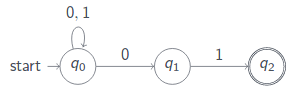
\includegraphics[scale=0.5]{Immagini/NFA.png}
\end{figure}

Infatti questo non può essere un DFA perchè da $q_0$ se leggo 0 posso trovarmi
contemporaneamente in $q_0$ e $q_1$, in più da $q_1$ posso muovermi solo in $q_2$ 
e da $q_2$ non posso proprio muovermi.
Un automa a stati finiti non deterministici(NFA) è una quintupla $A=(Q, \Sigma, 
\delta, q_0, F)$ dove
\begin{itemize}
\item Q è un insieme finito di stati;
\item $\Sigma$ è un alfabeto finito;
\item $\delta$ è una funzione di transizione che prende in input (q,a) e 
restituisce un sottoinsieme di Q;
\item $q_0 \in Q$ è lo stato iniziale;
\item $F \in Q$ è un insieme di stati finali;
\end{itemize}
Anche per i NFA abbiamo una definizione rigorosa:
\begin{itemize}
\item \textbf{base}: $\widehat{\delta}(q, \varepsilon)={q}$;
\item \textbf{induzione}: $\widehat{\delta}(q,w)=\bigcup_{p \in \delta 
(\widehat{q},x)}^{} \delta(p,a)$;
\end{itemize}
Data una parola, il nostro automa potrà trovarsi in uno dei tanti stati
che siamo andati a calcolare.

\section{Equivalenza tra DFA e NFA}
NFA e DFA sono in grado di riconoscere gli stessi linguaggi e l'equivalenza si
dimostra mediante una \textbf{costruzione a sottoinsiemi}. Infatti, dato un NFA
$N=(Q_N, \Sigma, q_0, \delta_N, F_N)$ costruiremo un DFA $D=(Q_D, \Sigma, {q_0}, 
\delta_D, F_D)$ tale che L(D)=L(N).
Ogni stato del DFA, $Q_D$ corrisponde ad un insieme di stati dell'NFA.
\textit{Uno stato del DFA $F_D$ è finale se c'è almeno uno stato finale
corrispondente all'NFA}. La funzione di transizione $\delta_D$ percorre tutte le
possibili strade. Ad esempio: 

\begin{figure}[h]
\centering 
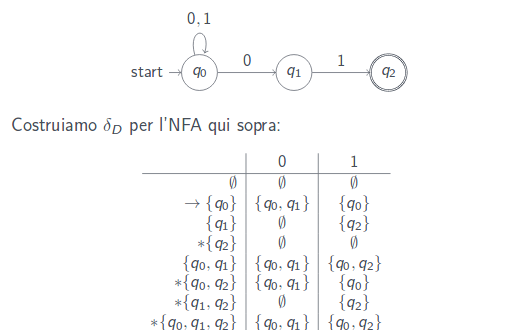
\includegraphics[scale=0.5]{Immagini/equivalenza1.png}
\end{figure}

\begin{figure}[h]
\centering 
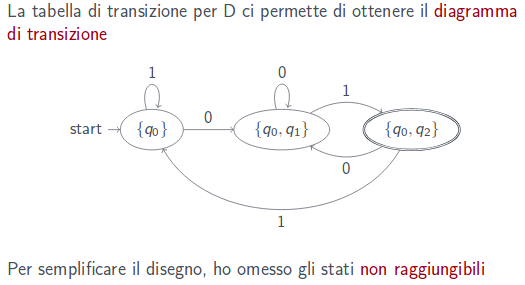
\includegraphics[scale=0.5]{Immagini/equivalenza2.png}
\end{figure}

\begin{thm}
Sia D il DFA ottenuto da un NFA N con la costruzione a sottoinsiemi. Allora
L(D)=L(N).
\end{thm}

\begin{thm}
Un linguaggio L è accettato da un DFA se e solo se è accettato da un NFA.
\end{thm}

\section{NFA con epsilon-transizioni}
Le epsilon-transizioni vengono usate per muovere l'automa di stato anche se non
viene dato nessun simbolo in input.
Un automa a stati finiti non deterministico con $\varepsilon$\textrm{-transizioni} ($
\varepsilon\textrm{-NFA}$)
è una quintupla $A=(Q, \Sigma, \delta, q_0, F)$ dove cambia solo

\begin{itemize}
\item \textbf{$\delta$} che è una funzione di transizione che prende in input uno 
stato in Q oppure un simbolo nell'alfabeto $\Sigma \cup \{\varepsilon\}$
\end{itemize}

L'eliminazione delle $\varepsilon$-transizioni procede per $\varepsilon$-chiusura 
degli stati, cioè prendendo tutti gli stati raggiungibili da q con una sequenza $
\varepsilon\varepsilon... \varepsilon$. L'$\varepsilon$-chiusura viene indicata con 
\textbf{ECLOSE(q)}.

\section{Equivalenza tra DFA e $\varepsilon$\textrm{-NFA}}
Per ogni $\varepsilon$\textrm{-NFA} E c'è una DFA D tale che L(E)=L(D), e viceversa.
Ogni stato del DFA corrisponde ad un insieme di stati chiuso per 
$\varepsilon$\textrm{-chiusura}.
Uno stato del DFA è finale se c'è \textbf{almeno} uno stato finale corrispondente 
nell'$\varepsilon$\textrm{-NFA}.















